\section{Current KLIPS input/output structure}

\subsection{output: ipsec\_tunnel\_start\_xmit}

\begin{enumerate}
	\item gather private information
	\item clone skb if necessary
	\item verify that packet is IPv4
	\item compute hard header length
	\item decrement TTL
	\item lookup in erouting table
	\item UDP port 500 exception
	\item start encapsulation loop
	\begin{enumerate}
		\item check for DROP or missing eroute
		\item check for REJECT eroute
		\item check for PASS eroute
		\item check for HOLD eroute
		\item check for TRAP eroute, signal PF\_KEY, swap to HOLD eroute
		\item acquire lock for walking tdb chain
		\item calculate headroom required for chain
		\begin{enumerate}
			\item check if SA is in larval, drop
			\item check if SA is dead, drop
			\item check if replay overflowed, expire SA
			\item check if lifetime counters have overflowed, expire SA
			\item switch on protocol type, to calculate headroom size.
			\begin{enumerate}
				\item if ESP switch on protocol type to calculate tailroom size.
			\end{enumerate}
		\end{enumerate}

		\item calculate mtudiff, send ICMP fragment needed. Mark ``note2''

		\item hack MSS if desired

		\item copy upper (layer 2) header to safety if it was present

		\item check if data fits in existing skb, else expand.
		\item apply grouped transforms
		\begin{enumerate}
			\item apply disaster of \#ifdefs.
			\item switch by protocol type, calculate headroom for this stage
			\begin{enumerate}
				\item if ESP, then switch by cipher get headroom
				\item if ESP, then switch by hash to get tailroom
			\end{enumerate}
			\item double check (not in NDEBUG) if there is enough headroom
			\item push the data ahead
			\item double check (not in NDEBUG) if there is enough tailroom
			\item extend the data behind
			\item see if packet has become too long (bigger than 64K)
			\item finally move the plaintext as appropriate
			\item switch on protocol type
			\item case: ESP
			\begin{enumerate}
				\item switch on cipher type, prepare IV
				\item prepare self-describing padding
				\item switch on cipher type, do encryption
				\item switch on cipher type, update IV
				\item switch on hash type, do authentication
			\end{enumerate}
			\item case: AH
			\begin{enumerate}
				\item prep replay info, headroom
				\item switch on hash type, do authentication
			\end{enumerate}
			\item case: IPIP, apply encap
			\item case: IPCOMP
			\begin{enumerate}
				\item call skb\_compress
				\item do some debugging
			\end{enumerate}
			\item recalculate header checksum
		\end{enumerate}
		\item lookup eroute by new outer header, if we found
			something and the src/dst have changed
	\end{enumerate}
	\item send ICMP if packet has become too big
	\item re-apply link layer header if there was one.
	\item attempt to re-route the packet
	\item drop packet if new route leads to us again.
	\item do connection tracking
	\item do netfilter localout output call
	\item call ip\_send or IP\_SEND depending on kernel version
\end{enumerate}

\subsubsection{Comments upon problems/limitations of transmit}

\subsection{input: ipsec\_rcv}

\begin{enumerate}
	\item increment module use count
	\item verify skb and data is not NULL
	\item verify hard header length
	\item clone (COW) if necessary
	\item a number of poorly documented ``assertions''
	\item verify protocol number against packet and against protocol structure
	\item verify that protocol is AH, COMP or ESP.
	\item lookup each ipsecX device to determine which one has been bound 
		to the receiving device. Grab ipsecprv device info.
	\item if no device found, warn, but do not die
	\item begin decap loop
		\begin{enumerate}
		\item lock tdb if this is first time through
		\item verify that length is appropriate multiple if ESP
		\item switch on protocol type, grab SPI value from appropriate place
		\item format sa with satoa. (not found in code)
		\item if AH, then determine AH header length, find next protocol value, and
			verify against expected length of AH header.
		\item get spin lock if required
		\item if IPCOMP
		\begin{enumerate}
			\item check if IPCOMP is out most header, (not yet supported)
			\item advance the tdb pointer and, if doing inbound policy
				check, then check SPI value. Complain if not matched.
			\item decompress packet, reset ip header pointer to new
				value, loop (via continue) 
		\end{enumerate}
		\item lookup tdb based upon SA. \code{gettdb}
		\item complain if no tdb
		\item if doing inbound policy check
		\begin{enumerate}
			\item check that outer source matches one on packet.
			\item check that this tdb is the expected next from
				previous. (forward check) 	
			\item check that this tdb expects to be attached to
				previous. (reverse check) 
		\end{enumerate}
		\item check if tdb state is larval, skip
		\item check if tdb state is dead, complain
		\item check lifetime (bytes - soft/hard, addtime - soft/hard, usetime -
			soft/hard, packet count - soft/hard). Expire TDB,
			tell pfkey if limit exceeded.
		\item pick authlen, switch on auth type (MD5, SHA1)
		\item switch on protocol type (ESP, AH only) and set up authenticator
		\item check sequence number to see if replay window rolled, if so expire
		\item check out replay window, dropping if it is a replay
		\item verify authenticator, check if there was
			authentication, switch on type 
		\begin{enumerate}
			\item MD5, call MD5Update and friends, checking if
				ESP or AH was involved 
			\item SHA1, call SHA1Update and friends, checking if ESP or
				AH was involved	 
			\item none, do nothing
		\end{enumerate}
		\item check authenticator for NULL (which would imply not AH
			or ESP above) 
		\item compare authenticator against hash, complain if failed
		\item update the replay window
		\item switch on protocol type
		\begin{enumerate}
			\item if ESP
			\begin{enumerate}
				\item switch on encryption algorithm
				\begin{itemize}
					\item if 3DES, then find IV and set header length
					\item otherwise, fail
				\end{itemize}
				\item locate ciphertext based upon header length
				\item switch on encryption algorithm
				\begin{itemize}
					\item if 3DES, verify data length
						multiple of 8 and decrypt. 
					\item no otherwise clause
				\end{itemize}	
				\item find next header type
				\item find padding 
				\item verify padding
			\end{enumerate}
			\item if AH, do nothing
		\end{enumerate}
		\item update protocol number in header (why?)
		\item switch on protocol type
		\begin{enumerate}
			\item if ESP, the memmove as appropriate for ESP,
				skb\_pull() to compact, and then skb\_trim.
			\item if AH, then memmove as appropriate for AH, skb\_pull().
		\end{enumerate}
		\item update skb pointers to parts of packet.
		\item nuke any options that skb knew about, or skb->proto\_priv (2.2+)
	\end{enumerate}
	\begin{enumerate}
		\item recalculate the header checksum
		\item set the sbk protocol type to IP over ethernet
		\item advance tdb pointers
		\item if doing inbound policy check
		\begin{enumerate}
			\item verify that backward policy agrees with forward policy
			\item check if next protocol field is not one we know about
			\begin{enumerate}
				\item complain that policy was not complete
			\end{enumerate}
		\end{enumerate}
		\item update ipcomp ratio counters if IPCOMP was involved, but this
			stage is not IPCOMP
		\item update the lifetime values in bytes, packets, and last used
			time.
		\item loop again if ESP, AH or IPCOMP
	\end{enumerate}

	\item if original chain was IPCOMP, then advance tdb chain once (Why?)
	\item if there is one last tdb
	\begin{enumerate}
		\item verify that last protocol type was IPIP (no transport
			supported here)
		\item if doing inbound policy checks
		\begin{enumerate}
			\item advance tdbnext with inext, and complain if
				non-NULL. (i.e. check that this was last tdb)
			\item verify source IP address matches tdb source
		\end{enumerate}
		\item update lifetimes for this tdb
		\item if skb data len is too small for header length,
			complain
		\item pull up new header into skb
		\item advance ip pointer to inner header
		\item update raw header pointer
		\item zero protocol options
		\item update layer 2 protocol info to IP over Ethernet
		\item reset checksum info
	\end{enumerate}
	\item if we are doing EROUTE checking (i.e. tunnel exit checking)
	\begin{enumerate}
		\item setup for look up by src/dst in eroute table, checking
			for IPIP header.
%		didn't we already advance ipp above? why are we looking in
%		a tunnel that we didn't make?
		\item lock eroute table, lookup eroute
		\item record info we need and unlock
		\item if we found what we need, then lock, and lookup policy
			information by new said block.
		\item if no tdb found, then we drop packet
		\item walk policy\_tdb chain, look for last one
		\item compare against tdb that we just used, complain if not
			the same.	
	\end{enumerate}
	\item unlock tbd
	\item update stats if appropriate
	\item release packet destination 
	\item if there was a layer 2, copy it back into place
	\item do inbound policy checks if it was IPCOMP 
% WHY HERE?
	\item do connection tracking
	\item drop packet back into bottom half queue
\end{enumerate}

\subsubsection{Comments upon problems/limitations of receive}

\section{KLIPS1 static structure}

\begin{figure}
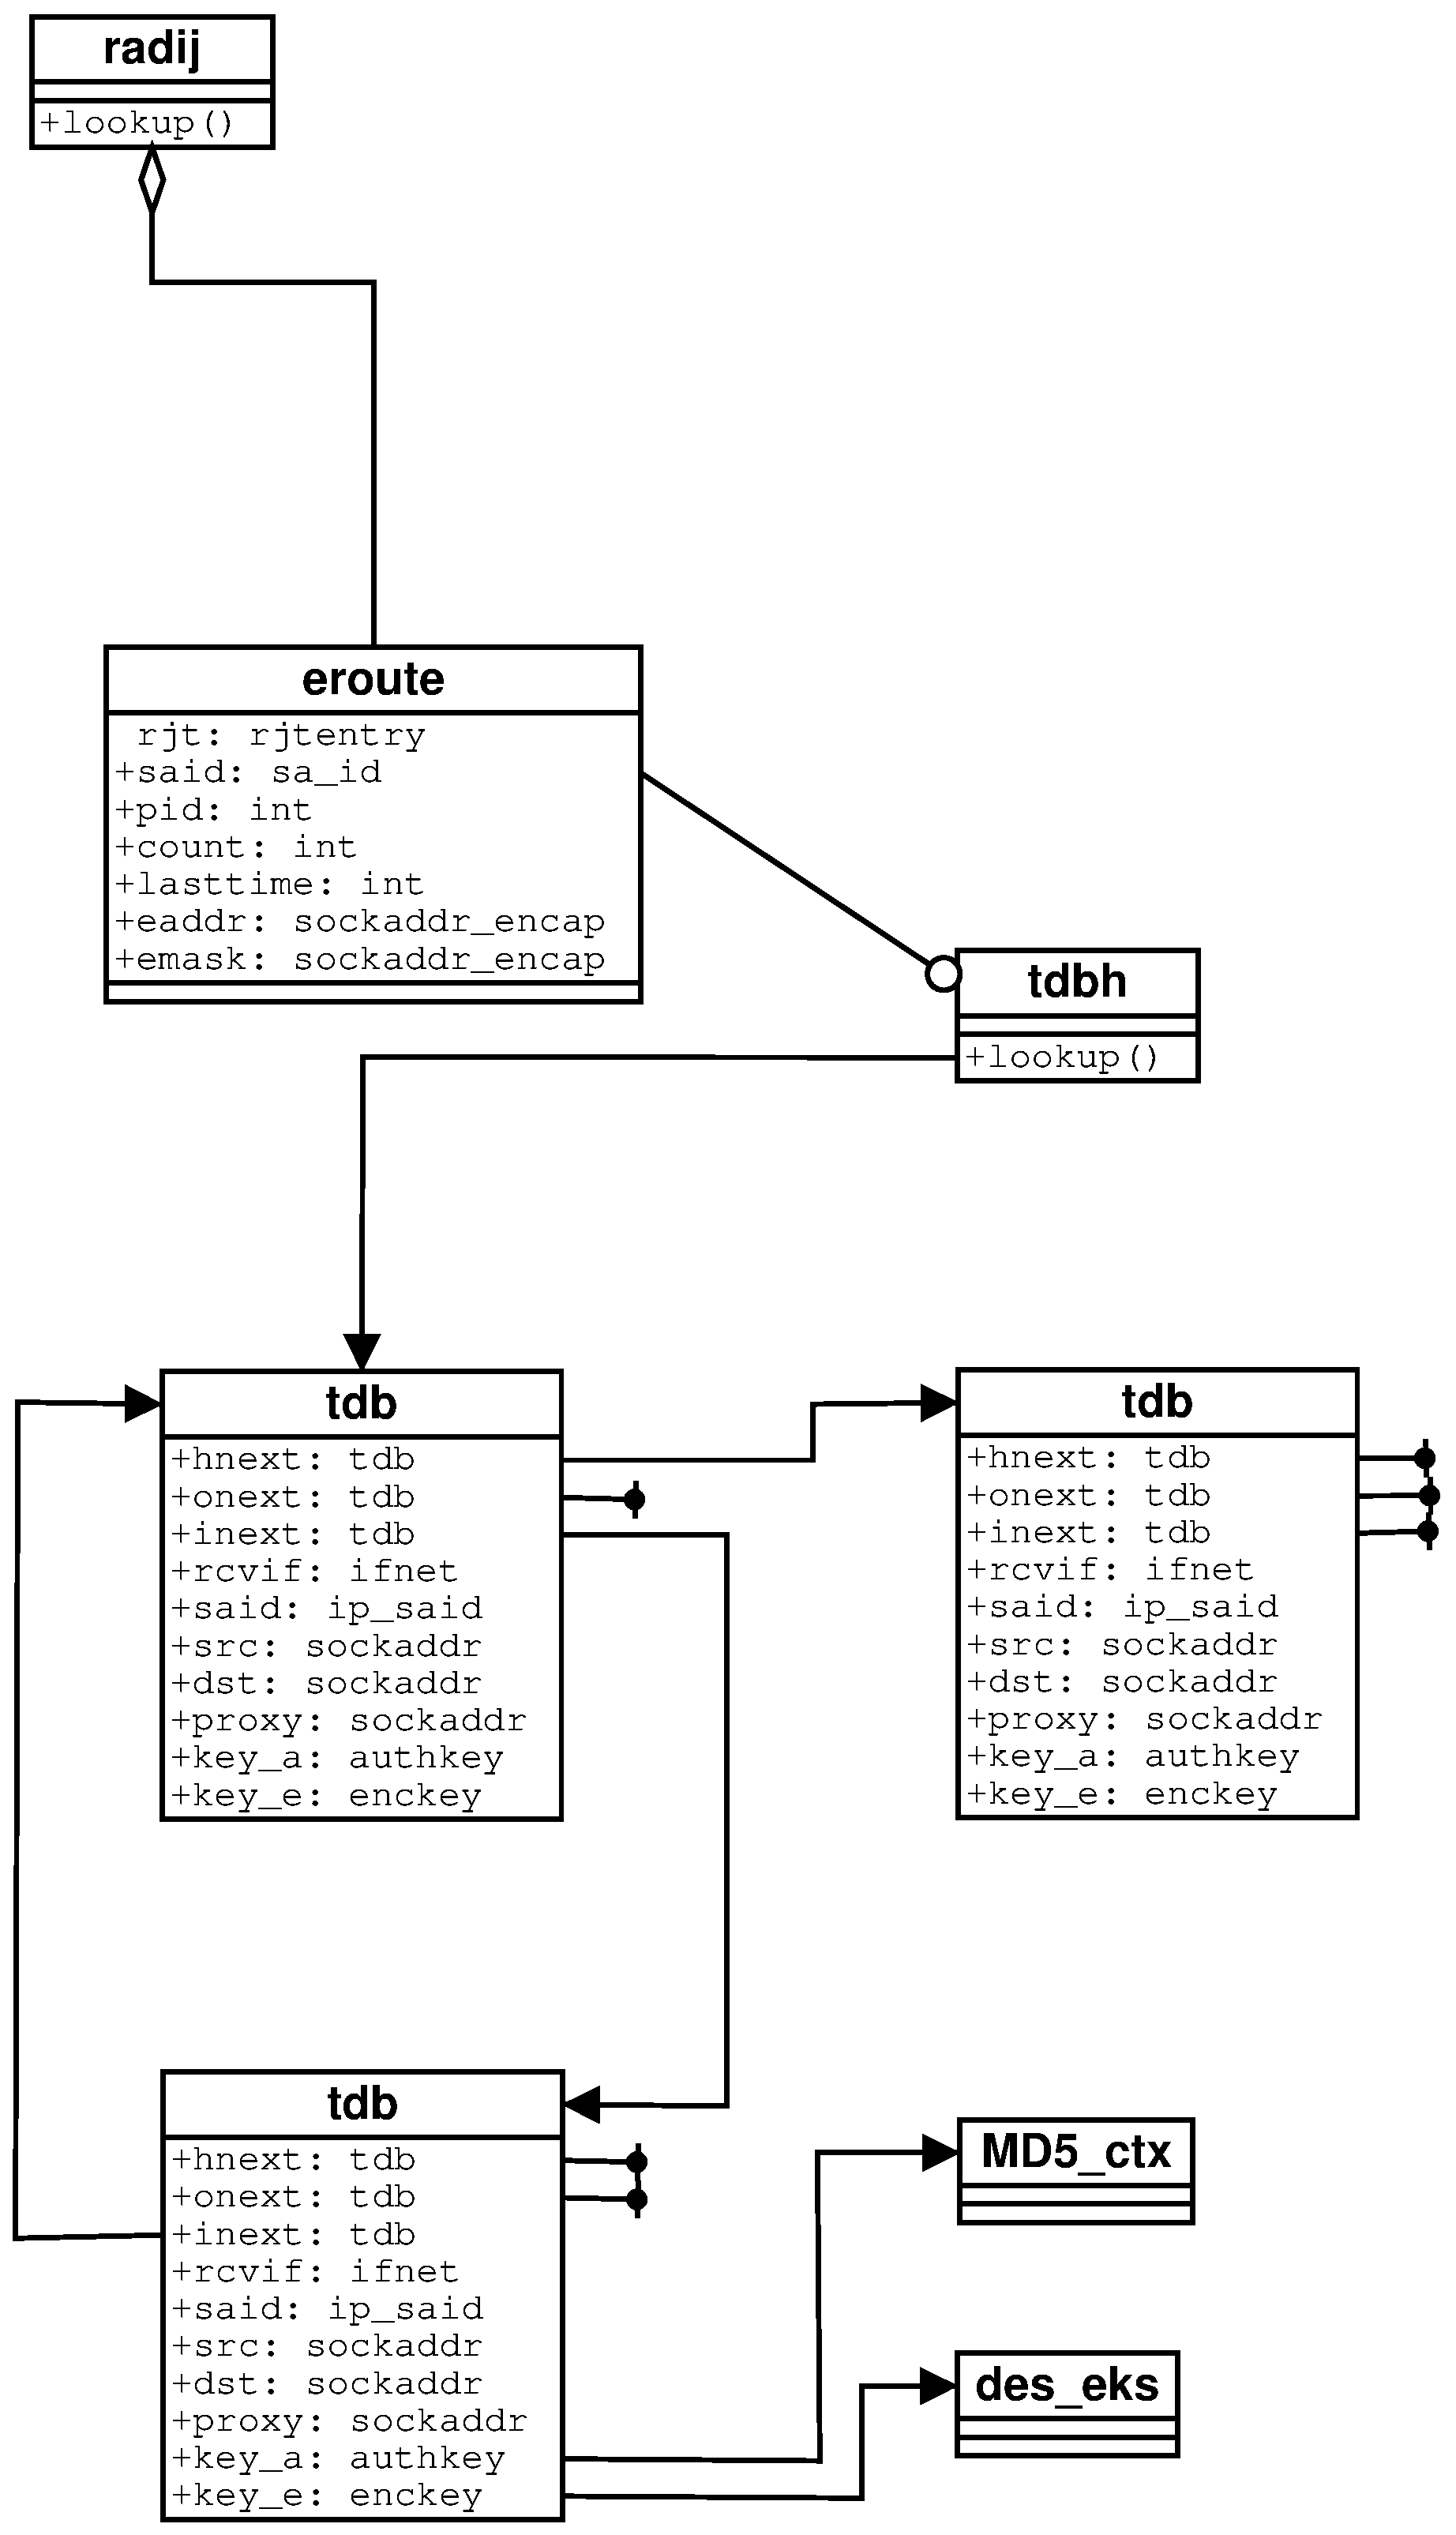
\includegraphics[height=6in,width=6in]{diagrams/klips1_tdb.eps} 
\label{KLIPS1 structures}
\end{figure}

\subsection{klips1 radij}

The \code{radij} module is an adaptation of the BSD \code{radix.c} code. It
has been consistently renamed to as to coexist with \code{radix.c}. It
implements a netmask aware patricia tree on blocks of data.

An explanation explains that the pronounciation is almost the same since the
``j'' is to be pronounced like the Greek chi.

\subsection{klips1 eroute}

An eroute entry describes an entry in the security policy database. The
\code{eroute} currently only includes selectors for source and destination address.

\subsection{klips1 tdbh}

This is an array of pointers to \code{struct tdb} structures. It serves as
a root for chained hash buckets. It is an open hash.

These are managed by the code in \code{ipsec\_xform.c}. These provide a
mapping from a \code{struct sa\_id} to a \code{struct tdb} based upon SPI,
protocol and destination address. 

The entries in each bucket are linked together using the \code{tdb\_hnext}
field.

\subsection{klips1 tdb}

This structure represents all the information associated with a single
transform. In the case that multiple transforms may be chained together, they 
are chained together using \code{tdb\_inext} and \code{tdb\_onext}. The ``i''
and ``o'' are short for inner and outer. Thinking of the resulting packet as
an onion, these pointers describe transforms towards the {\bf i}nner and {\bf 
o}uter directions.

\subsection{klips1 md5\_ctx}

This stores the key context for the MD5 authentication routines. This
structure is different from the \code{MD5\_CTX}, in that this is the HMAC
version and contains an inner and outer \code{MD5\_CTX}.

\subsection{klips1 sha1\_ctx}

This block is not shown in the diagram, but serves an analogous function to
\code{md5\_ctx}. 

\subsection{klips1 des\_eks}

This block contains a DES key schedule (this is not equivalent to a DES key,
but has been scheduled already). Note that this is really a container
and is assumed to be of the proper size. The DES routines actually take a
\code{des\_cblock} as input.



	
	
		
		
	
	
